\chapter{Codierungstheorie}

\section{Grundbegriffe und einfache Beispiele}

\subsection{Codierung} (Kanalcodierung)\\
Sicherung von Daten/Nachrichten gegen zuf\"allig auftretenden Fehler bei Speicherung/\"Ubertragung.\\
\begin{figure}[h]
	\centering
	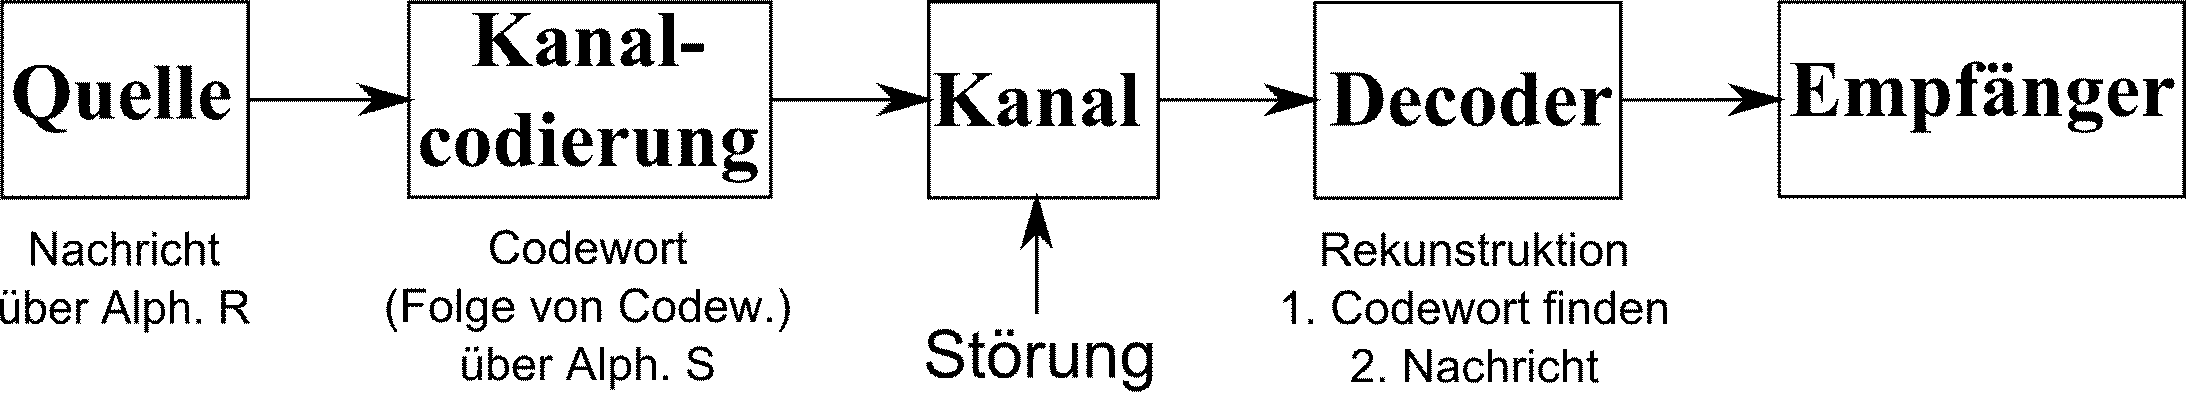
\includegraphics[width=15cm]{./img/codierung_schaubild.png}
	\caption{Schaubild der Codierung}
	\label{img:Schaubild Codierung}
\end{figure}

\subsection{Ziele}
\begin{itemize}
	\item M\"oglichst viele Fehler erkennen und gegebenenfalls korrigieren. %ABKUERZUNG
	\item Aufwand f\"ur Codierung und Decodierung m\"oglichst gering.
\end{itemize}

\section{Grundprinzip} Hinzuf\"ugen von Redundanz\\
\\
Es gibt zwei Typen um Redundanz zu erzeugen.
\subsection{FEC-Verfahren (Forward Error Correction)}
Aufgetretene Fehler sollen erkannt \underline{und} korrigiert werden.\\
Vorteil: keine Verz\"ogerung der \"Ubertragung aber ggf. gro\ss e Redundanz notwendig.

\subsection{ARQ-Verfahren (Automatic Repeat Request)}
Aufgetretene Fehler sollen erkannt werden, werden nicht korrigiert. Stattdessen  wiederholt die \"Ubertragung beim Sender anfordern.\\
\\
Vorteil: geringe Redundanz, aber Verz\"ogerung.\\
\\
\subsubsection{Beispiele}
\subsection{Parity-Check-Codes}
z.B. Nachrichten: 00, 01, 10, 11\\
\\
Codierung: 00 $\rightarrow$ 000\\
01 $\rightarrow$ 011\\
10 $\rightarrow$ 101\\
11 $\rightarrow$ 110\\
(gerade Anzahl von Einsen in den Codew\"ortern)\\
\\
1 Fehler wird erkannt, nicht korrigiert.\\
2 Fehler werden nicht erkannt.

\subsection{Wiederholungscode}
Nachrichten wie in 1.\\
\\
Codierung: 00 $\rightarrow$ 000000
01 $\rightarrow$ 010101\\
10 $\rightarrow$ 101010\\
11 $\rightarrow$ 111111\\
(3-Fache Wiederholung)\\
\\
1 Fehler wird erkannt und korrigiert.\\
\underline{01}01\underline{01} $\rightarrow$ 010101 $\rightarrow$ 01 \\

Nachrichten wie in 1.
Codierung: 00 $\rightarrow$ 00000\\
01 $\rightarrow$ 01101\\
10 $\rightarrow$ 10110\\
11 $\rightarrow$ 11011\\
\\
Je zwei Codew\"orter unterscheiden sich an mindestens 3 Positionen.\\
Angenommen 1 Fehler tritt bei \"Ubertragung auf. Dann gibt es genau ein Codewort, dass sich vom empfangenen Wort an genau einer Stelle unterscheidet; in das wird decodiert.\\
\\
Muss immer Ungerade unterschiede in Codew\"ortern sein. Bei 5 diffs sind 2 Fehler korrigierbar.
\subsection{(ehmaliger) ISBN-Code}
International Standard Book Number\\
\\
10-Stelliger Code\\
Erste 9 Ziffern haben inhaltliche Bedingung ($\entspricht$ Nachricht)\\
10. Ziffer: Pr\"ufziffer\\
\\
Beispiel: 3-540-26121-? (Land - Verlag - Buchnummer - Pr\"ufziffer)\\
\\
Uncodierte W\"orter sind gebildet \"uber $R=\{0, \ldots, 9\}$\\
Codierte W\"orter sind gebildet \"uber $S=\{0, \ldots, 9, X\}$\\
\\
ISBN-Wort $C_{10}C_9\ldots C_2C_1$\\
$C_{10}\ldots C_2$ inhaltliche Bedingung, $C_1$ wird so gew\"ahlt, dass
\[
	\sum^{10}_{k=1} k \cdot C_k \equiv 0 (\md 11)
\]

$10\cdot C_{10}+\ldots + 2\cdot C_2 + C_1 \equiv 0(\md 11)$ falls $C_1 = 10$ so setzte $C_1 = X$\\
$C_1$ vom Beispiel ausrechnen.\\
\\
$ 10\cdot 3+9\cdot 5+8\cdot 4+7\cdot 0+6\cdot 2+5\cdot 6+4\cdot 1+3\cdot 2+2\cdot 1+C_1 = 0 (\md 11)$\\
$ 161 + C_1 = 0 (\md 11) \Rightarrow C_1 = 4$\\
\\
\"Andern einer Ziffer wird erkannt:\\
$C_{10} C_9\ldots C_2 C_1 \rightarrow\ C_i$ wird $X_i \neq C_i$ ersetzt\\
$C_{10} \ldots C_{i+1} X_i C_{i-1} \ldots C_1$
\[
	\sum^{10}_{k=1, k \neq i} k \cdot C_k + i \cdot x_i = 
	\underbrace{\sum^{10}_{k=1, k \neq i} k \cdot C_k}_{\equiv 0 (\md 11)}
	\overbrace{
			\underset{\underset{\nequiv 0 (\md 11)}{\uparrow}}{i} 
			\cdot (\underbrace{x_i-c_i}_{\nequiv 0 (\md 11)}) 
	}^{\nequiv 0 (\md 11)}
	\nequiv 0(\md 11)	
\]
Fehler wird erkannt, Korrektur nicht m\"oglich.\\
\\
$3-540-26121-4 \equiv 0(\md 11)$\\ \\
$\left.
\begin{matrix}
	3-540-26121-\mathbf{6} \\
	3-540-2612\mathbf{2}-4
\end{matrix}
\right\} \text{Pr\"ufsumme 2.}
$\\

Vertauschung von Zwei Ziffern wird erkannt.\\
$C_i$ und $C_j$ vertauscht.\\
O.B.d.A $C_i \neq C_j$\\
$C_{10} \ldots \underset{\stackrel{\uparrow}{i}}{C_j} \ldots \underset{\stackrel{\uparrow}{j}}{C_i} \ldots C_1$\\
\[
	\sum^{10}_{k=1, k\neq i,j} k \cdot C_k + i \cdot 	C_j + j \cdot C_i
	= \sum^{10}_{k=1} k \cdot C_k + i(C_j-C_i)+j(C_i-C_j)
\]
\[
	= 
	\underbrace{\sum^{10}_{k=1} k \cdot C_k}_{\equiv 0 (\md 11)}
	 + 
	 \underbrace{(C_j-C_i)}_{\nequiv 0 (\md 11)}
	 \underbrace{(i-j)}_{\nequiv 0 (\md 11)}
	 \nequiv 0 (\md 11)
\]
Vertauschung wird durch gewichtete Quersummen erkannt.


\subsection{EAN-13-Code}
European Article Number\\
13-Stelliger Code, erste 12 Ziffer sind inhaltlich festgelegt.\\
13. Ziffer ist Pr\"ufziffer.\\
$R=S=\{ 0, \ldots, 9\}$ \\
$C_1 \ldots C_{12}C_{13}$\\
\\
$C_1 \ldots C_{12}$ inhaltliche Angabe (in der Regel):\\
$C_1C_2$ Herstellerland (40-43 Deutschland)\\
$C_6 \ldots C_7$ Hersteller
$C_8 \ldots C_12$ interne Produktions Nummer\\
\\
$C_{13}$ so gew\"ahlt, dass\\
\[
	C_1 + 3\cdot C_2 + C_3 + 3\cdot C_4 + \ldots + 3\cdot C_{12} + C_{13} \equiv 0 (\md 10)
\]
$x \rightarrow 3x$ Permutation auf $\Z_{10} (\md 10)$, da ggT(3,10)=1\\ %FORMATTING vom ggT?
1 Fehler wird erkannt. Vertauschung in der Regel nicht erkannt. \\
\\
\"Ubersetzung in Barcode: \\
$C_1 C_2 \ldots C_7 C_8 \ldots C_{13}$\\
\\
Jede der Ziffern $C_2, \ldots, C_{13}$ wird durch einen 0-1-String der L\"ange 7 bin\"ar codiert. \\
$0 \entspricht$ wei�er Balken, $1 \entspricht$ schwarzer Balken. \\
Codierung sorgt daf\"ur, dass nie mehr als 4 wei�e oder schwarze Balken nebeneinander stehen. \\

\newpage

\begin{figure}[h]
	\centering
	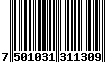
\includegraphics{./img/ean13.png}
	\caption{EAN-13 Barcode}
	\label{img:EAN-13 Barcode}
\end{figure}

Schmalen Balken in Mitte und am Rand, sind nur Abtrennzeichen, die nichts mit EAN zu tun haben und nur beim einscannen helfen.\\
5 zu $0110001_2$ \\
\\
$C_2,\ldots, C_7$ werden nach Code A oder Code B codiert. $C_1$ bestimmt welcher dieser beiden Codes verwendet wird. \\
$C_8,\ldots, C_{13}$ werden nach Code C codiert.\\
$C_1$ ergibt sich aus der Art der Codierung von $C_2,\ldots,C_7$

%Table shit here
\begin{center}
	\begin{tabular}{| c | c | c | c | p{2cm} |}
	\hline
	 &\multicolumn{2}{|c|}{\textbf{Ziffern $\mathbf{C_2 - C_7}$}} & \textbf{Ziffern $\mathbf{C_8 - C_{13}}$} & \textbf{bestimmt durch} $\mathbf{C_1}$ \\
	\hline
	\textbf{Zeichen} & \textbf{Code A} & \textbf{Code B} & \textbf{Code C} & \textbf{Code D}\\
	\hline
	\textbf{0} &	0001101 &	0100111 &	1110010 &	AAAAAA\\
	\textbf{1} &	0011001 &	0110011 &	1100110 &	AABABB\\
	\textbf{2} &	0010011 &	0011011 &	1101100 &	AABBAB\\
	\textbf{3} &	0111101 &	0100001 &	1000010 &	AABBBA\\
	\textbf{4} &	0100011 &	0011101 &	1011100 &	ABAABB\\
	\textbf{5} &	0110001 &	0111001 &	1001110 &	ABBAAB\\
	\textbf{6} &	0101111 &	0000101 &	1010000 &	ABBBAA\\
	\textbf{7} &	0111011 &	0010001 &	1000100 & 	ABABAB\\
	\textbf{8} &	0110111 &	0001001 &	1001000 &	ABABBA\\
	\textbf{9} &	0001011 &	0010111 &	1110100 &	ABBABA\\
	\hline
	\end{tabular}
\end{center}

\noindent Codew\"orter von Code A,B oder C kommen nur einmal vor. Daher treten nie mehr als 4 gleiche Balken nebeneinander auf. \\







\section{Blockcodes}
\[
\begin{matrix}
	00 & \rightarrow & 00000\\
	01 & \rightarrow & 01101\\
	10 & \rightarrow & 10110\\
	11 & \rightarrow & 11011
\end{matrix}
\]

\subsection{Definition}

$S$ endl. Menge (=Alphabet), $n \in \N$. \\
Ein Blockcode $\mathcal{C}$
der (Block-)L\"ange $n$ \"uber $S$ ist Teilmenge von $S^n=\underset{\longleftarrow \ \  n\ \  \longrightarrow}{S \times \ldots \times S}$ \\ % Pfeilspa� <- n -> \times
\\
Elemente von $\mathcal{C}$ hei�en \textbf{Codew\"orter}. \\
Ist $\left| S \right| = 2$ (i.d.R. $S=\lbrace 0,1 \rbrace$, so \textbf{bin\"ar} Code.\\
$\left| \mathcal{C} \right| = m$, so ist $m \leq \left| S \right| ^ n$. \\
\\
Dann lassen sich $n$ Informationssymbole (oder Strings von Informationssymbolen) codieren (Codierungsfunktion). Folge von Informationssymbolen (oder Strings) werden dann in Folge von Codew\"ortern codiert.

\subsection{Definition: Hamming-Abstand}
$S$ endl. Alphabet, $n \in \N$. \\
$a,b \in S^n$ $a=(a_1, \ldots, a_n)$, $b=(b_1, \ldots, b_n)$ \\
$d(a, b)= \sharp \lbrace i : a_i \neq b_i \rbrace$ \\
\textbf{Hamming-Abstand} von $a$ und $b$. \\
(Richard W. Hamming, 1915-1998, Begr\"under der Codierungstheorie)\\
\subsubsection{Eigenschaften}
\begin{description}
	\item[a)] $d(a,b)=0 \Leftrightarrow a=b$
	\item[b)] $d(a,b)=d(b,a)$
	\item[c)] $d(a,b) \leq d(a,c) + d(c,b)$ (Dreiecksungleichung) \\
					($a_i \neq b_i \Rightarrow a_i \neq c_i$ oder $b_i \neq c_i$) 
	\item[d)] Wenn $(S,+)$ komm. Gruppe, dann auch $S^n$\\
					$[ (a_1,\ldots a_n) + (b_1, \ldots b_n) = (a_1+b_1,\ldots, a_n+b_n)]$\\
					$d(a,b)=d(a+c,b+c)$ (Translationsinvarianz)				
\end{description}

\noindent Also: Wird $x \in \mathcal{C}$ gesendet und $y \in S^n$ wird empfangen und $d(x,y)=k$, so sind $k$ Fehler aufgetreten.
\subsection{Definition}
\subsubsection{a) Hamming-Decodierung}
f\"ur Blockcode $\mathcal{C} \subseteq$ $S^n$ \\
Wird $y \in S^n$ empfangen, so wird $y$ zu einem Codewort $x' \in \mathcal{C}$ decodiert, das unter allen Codew\"ortern minimalen Hamming-Abstand zu $y$ hat.\\
\[
	d(x',y)=min\  d(x,y), x \in \mathcal{C}
\]
($x'$ muss nicht eindeutig bestimmt sein)	\\
z.B. $\mathcal{C}$ $ = \{ (0000), (1111) \}$\\
Empfangen: $0011$ $x'$ nicht eindeutig in diesem Fall.\\
\\
($\left| S \right | = 2$: Hamming-Decodierung ist bestm\"oglich, falls jedes Symbol in einem Codewort mit der gleichen Wahrscheinlichkeit $p < \frac{1}{2}$ ver\"andert wird und wenn jedes Codewort gleich wahrscheinlich ist.)\\

\subsubsection{b) Minimalabstand}
$\mathcal{C}$ Blockcode in $S^n$, Minimalabstand von $\mathcal{C}$: \\
\[
	d(\mathcal{C}) = min \  d(x,x')\mathbf{,}\ \  x,x' \in \mathcal{C}, x \neq x'
\]

(Ist $\left| \mathcal{C} \right| = 1$, so $d(\mathcal{C})=n$)\\
$[Bsp: \mathcal{C} = \lbrace (00000),(01101),(10110),(11011) \rbrace , d(\mathcal{C})=3]$\\

\subsubsection{c)} 
Ein Blockcode $\mathcal{C}$ ist \textbf{t-Felder-korrigierend}, falls $d(\mathcal{C}) \geq 2t+1$, und er hei�t \textbf{t-Fehler-erkennend}, falls $d(\mathcal{C}) \geq t+1$. \\
\\
Begr\"undung f\"ur die Bezeichnung in c) \\
"`Kugel"' vom Radius $t$ um $x \in \mathcal{C}: K_t(x) = \{y \in S^n: d(x,y) \leq t\}$\\
\\
Ist $d(\mathcal{C}) \geq 2t+1$, so sind Kugelm vom Radius $t$ um Codew\"orter disjunkt. \\
\\
Angenommen es existiert $y \in S^n$ mit $y \in K_t(x)\cap K_t(x')$, $x,x' \in \mathcal{C}, x \neq x'$. Dann $d(x,x') \leq d(x,y)+d(y,x') \leq t+t = 2t$. Widerspruch\\ %LIGHTNING ARROW \lightning
$x \in \mathcal{C}$ gesendet, $y$ wird empfangen, und angenommen maximal $t$-Fehler sind aufgetreten, dann $y \in K_t(x)$ und Abstand zu jedem anderem Codewort ist $> t$\\
$\Rightarrow$ Hamming-Decodierung ist korrekt.\\
$d(\mathcal{C}) \geq t+1$ und es treten maximal $t$ minimal $1$ Fehler auf, so ist $y$ kein Codewort.\\
\\
\textbf{Bsp}: 
\begin{description}
	\item[a)] $n$-fach Wiederholungscode \\
	$
	\begin{matrix} 
		S_n & \rightarrow & \underset{\longleftarrow \ \ n \ \ \longrightarrow}{S_1 S_1 \ldots S_1} \\ 
		\vdots \\
		S_k & \rightarrow & \underset{\longleftarrow \ \ n \ \ \longrightarrow}{S_k S_k \ldots S_k}
	\end{matrix}$\\
	\\
	$\mathcal{C}=\lbrace (s,s,\ldots,s): s \in S \rbrace \subseteq S^n$ \\
	$d(\mathcal{C})=n$ \\
	\\
	$\left\lfloor \frac{n-1}{2} \right\rfloor$-Fehler-korr.
	\item[b)] ISBN, EAN-Codes, $d(\mathcal{C})=2$, 1-Fehler-erkennend.
\end{description}

%WIP hier muss noch mehr verbessert werden
\section{Ab hier WIP (keine grundlegende Korrektur oder Versch\"onerung)}
\noindent
$d(\mathcal{C}) \geq 2 \cdot t + 1,\ \mathcal{C} \subseteq R^N$ \\
$K_t(x) \cap K_t(x')=\emptyset$ \\
$x, x' \in \mathcal{C},\ x \neq x'$ \\
$y$ empfangen, \\
- falls $y$ in $K_t(x)$ liegt f\"ur einen $x \in \mathcal{C}$, so wird $y$ nach $x$ decodiert (Korrekt, falls max. $t$ Fehler aufgetreten sind) \\
- falls $y$ in keiner $K_t(x)$ liegt, so kann es mehrere Codew\"orter geben mit gleichem min. Abstand zu $y$. (Dann keine eindeutige  Decodierung)

%Def
\noindent
Def: Code $\mathcal{C} \subseteq R^n$ hei�t perfekt, falls es ein $t \in \N_0$ gibt, mit der Eigenschaft:
\[
	R^n = \bigcup_{x\in \mathcal{C}} K_t(x) \ \text{u. $K_t(x) \cap K_t(x') = \emptyset$ f\"ur $x,x' \in \mathcal{C}, x \neq x'$}
\]
Dann ist $d(\mathcal{C})=2 \cdot t + 1$, falls $\left| \mathcal{C} \right| > 1$: \\
Ang. $d(\mathcal{C}) \leq 2\cdot t$. W\"ahle $x,x' \in \mathcal{C}, x \neq x'$, mit $d(x,x') = d(\mathcal{C}) \leq 2 \cdot t$. \\
W\"ahle $y \in R^n$ mit $d(x,y)=t,\ d(y,x')=t$\\
$y \in K_t(x) \cap K_t(x')$ % Widerspruchzeichen
\\
$d(\mathcal{C}) \leq 2 \cdot t + 1$ \\
W\"ahle $x \in \mathcal{C}$, w\"ahle $y \in R^n$ mit $d(x,y)=t+1$. Nach Vor. existiert $x' \in \mathcal{C}$ mit $y \in K_t(x')$. 
\[
	\begin{split}
		d(x,x') \leq d(x,y) + d(y,x') \leq t+1+t = 2 \cdot t + 1 \\
		d(\mathcal{C}) \leq 2\cdot t + 1
	\end{split}	
\]

\subsection{Gibt es perfekte Codes?}
Trivial Beispiele:
\begin{itemize}
	\item einelementige Codes (t=m)
	\item $\mathcal{C} = R^n$ (t=0) \\
				(Jedes Element ist ein Codewort)
	\item $n$-fache Wiederholungscode \"uber $Z_2$ \\
				$n=2 \cdot t +1$ \\
				$\mathcal{C} = \lbrace (0,\ldots,0),(1,\ldots,1)\rbrace$ % unter Pfeile <- n -> 
\end{itemize}

\subsection{Lemma}
$\left| R \right| = q,\ x \in R^n,\ t \in \N$ \\
Dann ist $\left| K_t(x) \right| = \sum_{i=0}^t (n,i)^{transponiert} \cdot (q-1)^i$ \\
$(n,i)^t=\frac{n\!}{i\! \cdot (n-i)\!}$ \\

\subsubsection{Beweis}
Abstand 0 zu $x$: 1 Word (n\"amlich $x$): $(n,0)^t \cdot (q-1)^0 =1$ \\
Abstand $i>0$ zu x: \\
Anzahl der Auswahl von $i$ Positionen aus $n$ Positionen: $(n,i)^t$ \\
An jeder Position $q-1$ \"Anderungsm\"oglichkeiten. \\
$\rightarrow$ insgesamt $(q-1)^i$ M\"oglichkeiten, \\
Anzahl der W\"orter vom Abstand $i$ von $x$: $(n,i)^t \cdot (q-1)^i$ \\
\subsubsection{Satz}
Sei $\mathcal{C}$ ein Code der L\"ange $n$ \"uber $R$, $\left| \mathcal{C} \right|> 1, \left|R\right| = q$. Sei $t \in \N_0$ maximal mit $d(\mathcal{C}) \geq 2 \cdot t + 1,\ t=\lfloor \frac{d(\mathcal{C})-1}{2}\rfloor$.
\begin{itemize}
	\item[a)] (Kugelpackungsschranke) \\
	$\left|\mathcal{C}\right| \leq \frac{q^n}{\sum_{i=0}^t (n,i)^{trans} \cdot (q-1)^i}$
	\item[b)] $\mathcal{C}$ ist perfekt $\Leftrightarrow$ in a) gilt Gleicheit, d.h. $\left|\mathcal{C}\right| = \frac{q^n}{\sum_{i=0}^t (n,i)^{trans} \cdot (q-1)^i}$
\end{itemize}

\noindent %Beweis
a)\\
$d(\mathcal{C}) \geq 2 \cdot t + 1$, daher $K_t(x) \cap K_t(x')=\emptyset,\ x\neq x',\ x,x' \in \mathcal{C}$  \\
$R^n \geq \bigcup_{x \in \mathcal{C}} K_t(x)$ \\
$q^n=\left|R^n\right|$ \\
$\left| \bigcup_{x \in \mathcal{C}} K_t(x) \right| = \sum_{x \in \mathcal{C}} \left| K_t(x) \right|$ \\
$=\left| \mathcal{C} \right| \cdot \sum_{i=0}^t (n,i)^{trans} \cdot (q-1)^i$\\
\\
b)\\
$\Rightarrow:d(\mathcal{C})=2 \cdot t +1$ \\
$R^n = \bigcup_{x \in \mathcal{C}} K_t(x) \Rightarrow \text{Gleicheit in a)}$\\
$\Leftarrow:$ Gleichheit $\Rightarrow R^n=\bigcup K_t(x) \Rightarrow \mathcal{C}$ perfekt.

%Teil 2 der Vorlesung

Bsp: Bin\"arer Hamming-Code der L\"ange 7 \\
$R=\Z_2=\lbrace 0,1 \rbrace$ $\mathcal{C}$ perfekt, $d(\mathcal{C})=3,\ \left| \mathcal{C} \right| = 16$ \\
$\mathcal{C} = \lbrace (C_1,\ldots,C_7) : C_i \in \Z_2,\ C_1 + C_4 + C_6 + C_7 = 0,\ C_2 + C_4 + C_5 + C_7 = 0,\ C_3 + C_5 + C_6 + C_7 = 0 \rbrace \subseteq \Z_2^7$ \\
$\mathcal{C}$ ist Unterraum von $\Z_2^7$ \\
$(C_1,\ldots,C_7) \in \mathcal{C},\ (C_1',\ldots,C_7') \in \mathcal{C}$ \\
$(C_1 + C_1',\ldots,C_7+C_7')\ \ (C_1+C_1') + (C_4+C_4') + (C_6+C_6') + (C_7+C_7') = 0$ \\
$dim(\mathcal{C})=4,\ C_4,C_5,C_6,C_7$ frei w\"ahlbar $\curvearrowright C_1,C_2,C_3$ festgelegt \\
Basis
\[
	\begin{split}
		(\ldots 1000) \rightarrow (1101000) \\
		(\ldots 0100) \rightarrow (0110100) \\
		(\ldots 0010) \rightarrow (1010010) \\
		(\ldots 0001) \rightarrow (1110001)
	\end{split}
\]
$\left| \mathcal{C} \right| =2^4 =16$\\
$d(\mathcal{C})=3:$\\
Ang. $d(\mathcal{C})=d$ W\"ahle $x,x' \in \mathcal{C}$ mit $d(x,x')=d$ Translationsinvarianz der Metrik: \\
$d=d(x,x')=d(x+x,x+x')=d(0,x+x')$ \\
$wt(x) = $ Anzahl der Einsen in $x$ \\
$= d(0,x)$. \\
$d(\mathcal{C}) = min wt(x)$. \\

Zeige: Jeder Vektor $\neq v$ in $\mathcal{C}$ enth\"alt mind. 3 Einsen.\\
$= 3$ weist man nach durch \"uberpr\"ufen aller 15 von 15 verschiedenen Codew\"ortern oder durch Analyse der Gleichung. \\
$(C_1,\ldots,C_7) \in \mathcal{C}$ Ang. $C_7=1$ \\
$\Rightarrow C_1+C_4+C_6=1$. Wenn alle Eins *check* \\%hier hacken
$C_1=1,C_4=C_6=0$\\
$C_4=1,C_1=C_6=0$\\
$C_6=1,C_1=C_4=0$\\
%verweis auf Menge von oben
Add $C_1+C_2+C_3+C_7=0$ \\
$C_1, C_2\ oder\ C_3 = 1$ \\
2. Fall: $C_7=1,C_4=1,C_1=0,C_2\ oder\ C_3=1$ \\
3. Fall: analog \\
1. Fall: $C_1=1,C_4=C_6=0$, o.B.d.A. $C_2=C_3=0 \Rightarrow C_5=1$

% jetzt gehts weiter
$d(\mathcal{C}) \leq 3,\ d(\mathcal{C})=3=2 \cdot 1 + 1$\\
Pr\"ufe nach, ob bei Kugelpackungsschranke Gleichheit gilt:\\
$\left|\mathcal{C}\right|=16$\\
$\left|\mathcal{C}\right| \leq \frac{q^n}{\sum_{i=0}^t (n,i)^{trans} \cdot (q-1)^i}=\frac{2^7}{1+(7,1)^t}=\frac{2^7}{2^3}=2^4=16$\\
$\mathcal{C}$ perfekt!
